% Diagram for the report (events). Build: see build.sh in this folder.
\documentclass[12pt]{standalone}
% Shared style of every diagram and chart in the report.
% Each agent keeps the same colour in every figure.
% The diagrams are drawn here, not in main.tex, so the report itself does not
% load TikZ: it includes the built PDFs and compiles within Overleaf's time limit.
\usepackage{amsmath,amssymb}
\usepackage{xcolor}
\usepackage{tikz}
\usetikzlibrary{positioning,arrows.meta,shapes.geometric,shapes.misc,fit,calc,backgrounds}
\usepackage{pgfplots}
\pgfplotsset{compat=1.18}

% Same text width as the report (A4, 30 mm + 20 mm margins), for the charts.
\setlength{\textwidth}{160mm}
\newcommand{\Rs}{Rs.\,}
\newcommand{\code}[1]{\texttt{\detokenize{#1}}}

\definecolor{ink}{HTML}{2B2B2B}
\definecolor{agAfill}{HTML}{E4F2E1}\definecolor{agAline}{HTML}{3E7D3A} % Agent 1 Document & Vendor
\definecolor{agBfill}{HTML}{FCEBD5}\definecolor{agBline}{HTML}{B8701D} % Agent 2 Approval & Inventory
\definecolor{agCfill}{HTML}{EEE4F4}\definecolor{agCline}{HTML}{6E4A8E} % Agent 3 Contract & Risk
\definecolor{agDfill}{HTML}{FBE4E4}\definecolor{agDline}{HTML}{A8474B} % Agent 4 Platform
\definecolor{infill}{HTML}{E8EDF6}\definecolor{inline}{HTML}{4F6188}    % infrastructure / data
\definecolor{exfill}{HTML}{F2F2F2}\definecolor{exline}{HTML}{6F6F6F}    % people and external systems
\definecolor{humfill}{HTML}{FFF6D6}\definecolor{humline}{HTML}{9A7B12}  % human decision points
\definecolor{chartA}{HTML}{9AA5B1}\definecolor{chartB}{HTML}{3F5E8C}    % chart: baseline / shipped

\tikzset{
  >={Stealth[length=2mm]},
  every picture/.style={font=\footnotesize, line width=0.6pt, draw=ink, text=ink},
  nohyph/.style={execute at begin node={\hyphenpenalty=10000\exhyphenpenalty=10000}},
  box/.style={nohyph, draw, rounded corners=2pt, align=center, inner sep=3pt, minimum height=8mm},
  agA/.style={box, fill=agAfill, draw=agAline},
  agB/.style={box, fill=agBfill, draw=agBline},
  agC/.style={box, fill=agCfill, draw=agCline},
  agD/.style={box, fill=agDfill, draw=agDline},
  infra/.style={box, fill=infill, draw=inline},
  ext/.style={box, fill=exfill, draw=exline},
  human/.style={box, fill=humfill, draw=humline},
  decision/.style={nohyph, diamond, aspect=2.2, draw=humline, fill=humfill, align=center, inner sep=1pt},
  flow/.style={->, draw=ink},
  dflow/.style={->, draw=ink, dashed},
  lbl/.style={font=\scriptsize\itshape, fill=white, inner sep=1pt},
  note/.style={font=\scriptsize\itshape, align=center},
}
\pgfplotsset{
  reportbars/.style={
    ybar, width=0.95\textwidth, height=6cm, ymin=0,
    enlarge x limits=0.18, bar width=11pt,
    ymajorgrids, grid style={draw=black!12},
    axis line style={draw=black!60}, tick style={draw=black!60},
    legend style={draw=none, font=\footnotesize, legend columns=-1, at={(0.5,1.03)}, anchor=south},
    tick label style={font=\footnotesize}, label style={font=\footnotesize},
    nodes near coords, every node near coord/.append style={font=\scriptsize},
    /tikz/every even column/.append style={column sep=0.6cm},
    legend image code/.code={\draw[#1, draw=none] (0cm,-0.1cm) rectangle (0.3cm,0.1cm);},
  },
}

\begin{document}
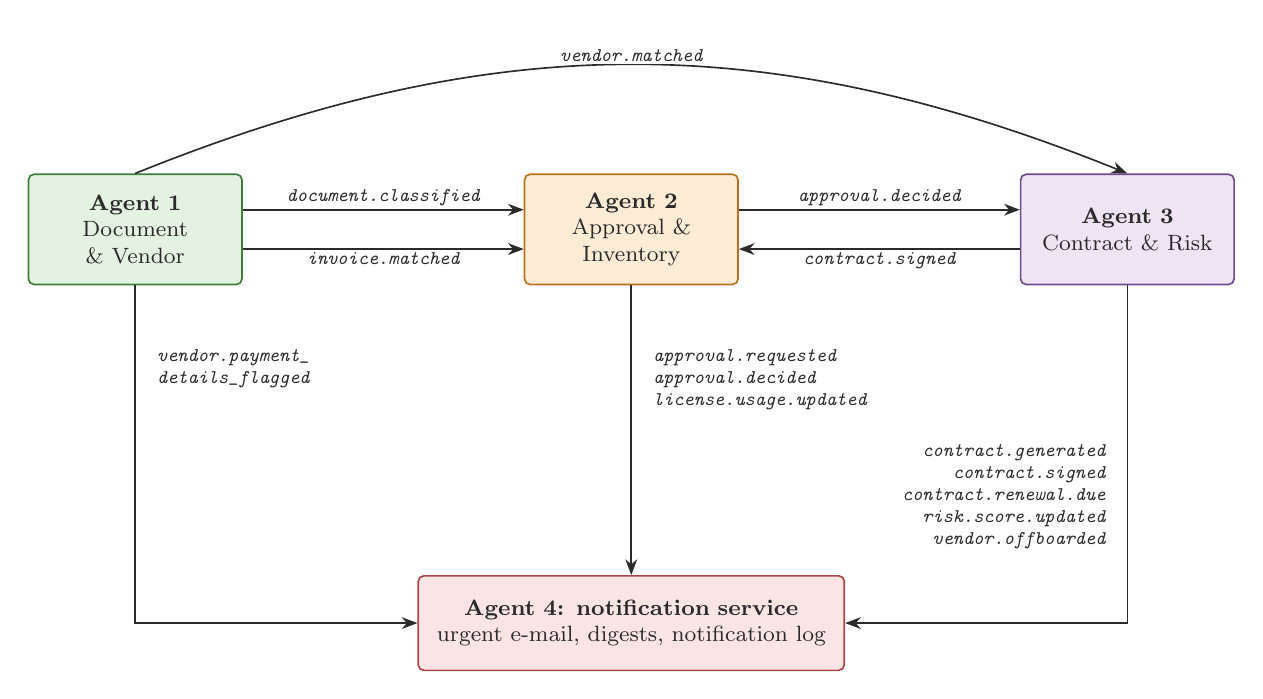
\begin{tikzpicture}
\node[agA, text width=2.5cm, minimum height=14mm] (a1) at (-6.3,0) {\textbf{Agent 1}\\Document \& Vendor};
\node[agB, text width=2.5cm, minimum height=14mm] (a2) at (0,0) {\textbf{Agent 2}\\Approval \& Inventory};
\node[agC, text width=2.5cm, minimum height=14mm] (a3) at (6.3,0) {\textbf{Agent 3}\\Contract \& Risk};
\node[agD, text width=5.2cm, minimum height=12mm] (nt) at (0,-5.0) {\textbf{Agent 4: notification service}\\urgent e-mail, digests, notification log};
\draw[flow] ([yshift=2.5mm]a1.east) -- node[lbl, above] {\code{document.classified}} ([yshift=2.5mm]a2.west);
\draw[flow] ([yshift=-2.5mm]a1.east) -- node[lbl, below] {\code{invoice.matched}} ([yshift=-2.5mm]a2.west);
\draw[flow] ([yshift=2.5mm]a2.east) -- node[lbl, above] {\code{approval.decided}} ([yshift=2.5mm]a3.west);
\draw[flow] ([yshift=-2.5mm]a3.west) -- node[lbl, below] {\code{contract.signed}} ([yshift=-2.5mm]a2.east);
\draw[flow] (a1.north) to[out=22, in=158] node[lbl, above] {\code{vendor.matched}} (a3.north);
\draw[flow] (a1.south) |- (nt.west);
\draw[flow] (a2.south) -- (nt.north);
\draw[flow] (a3.south) |- (nt.east);
\node[note, anchor=north west, align=left] at (-6.15,-1.4) {\code{vendor.payment_}\\\code{details_flagged}};
\node[note, anchor=north west, align=left] at (0.15,-1.4) {\code{approval.requested}\\\code{approval.decided}\\\code{license.usage.updated}};
\node[note, anchor=north east, align=right] at (6.15,-2.6) {\code{contract.generated}\\\code{contract.signed}\\\code{contract.renewal.due}\\\code{risk.score.updated}\\\code{vendor.offboarded}};
\end{tikzpicture}
\end{document}
